\chapter{Auswertung}
\label{chap:auswertung}

Nach dem Buch Software-Qualität von Peter Liggesmeyer
ist ein Qualitätsmerkmal, eine "Eigenschaft einer Funktionseinheit, anhand derer ihre \(\rightarrow\)
Qualität beschrieben und beurteilt wird, die jedoch keine Aussage über
den Grad der Ausprägung enthält. Ein Qualitätsmerkmal kann über mehrere Stufen in Teilmerkmale
verfeinert werden."\cite[S. 515]{SoftwareQualitaet} Typische Qualitätsmerkmale in der Softwareentwicklung
sind Korrektheit, Vollständigkeit, Sicherheit, Zuverlässigkeit, Verfügbarkeit und Robustheit \cite[S. 5]{SoftwareQualitaet}.
Die QA bietet sich besonders gut für Integrations- sowie End-to-End-Tests an. Diese testen
das Zusammenspiel der einzelnen Komponenten.


% Probleme: cookies verändern sich, Service Worker verändert sich, neue Felder in der Datenbank
% Frontend und Backend etc, also allen verschiedenen Services

\begin{figure}
    \label{figure:screenshotdeswebsocketdatenverkehrs}
    \begin{center}
    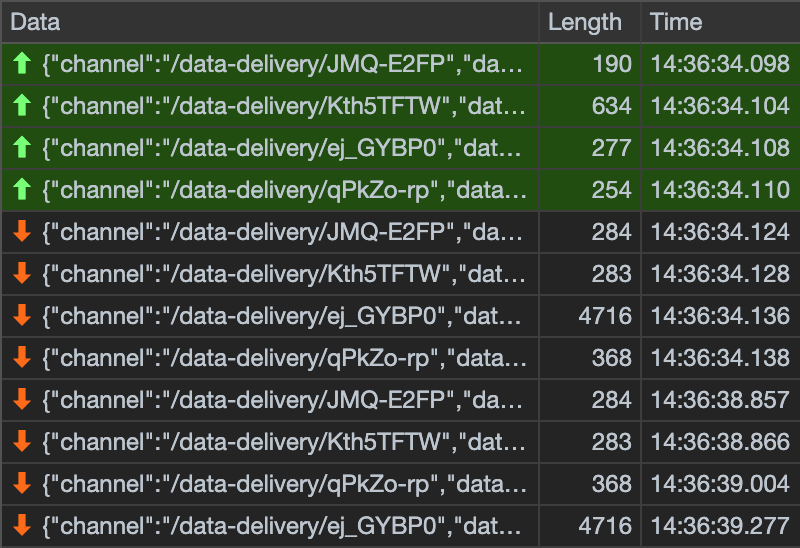
\includegraphics[scale=0.65]{img/screenshots/WebSocketTraffic}
    \end{center}
    \caption{Screenshot des WebSocket-Datenverkehrs}
\end{figure}
% Erkenntnis, Der Cache ist viel schneller, Cache ist O(1) wohingegen datenverarbeitung O(n) ist siehe
% anhand der größeren Anfrage

\section{Umgesetzte Anforderungen}
\label{sec:umgesetzteanforderungen}

\section{Testabdeckung}
\label{sec:testabdeckung}

\section{Lasttests}
\label{sec:lasttests}

\section{Skalierung der Services}
\label{sec:skalierungderservices}

\section{Übertragung}
\label{sec:uebertragung}

Steve Souders betont
in einem Vortrag über die Performance von JavaScript, dass ein Drittel der im Browser
geladenen First-Party-Scripts zwischen 90- und 100Kb nicht komprimiert werden.
Das liege daran, dass jQuery, eine der meistgenutztesten JS-Bibliotheken,
unkomprimiert circa bei 100Kb angesiedelt sei.\cite{SteveSoudersMakeJavaScriptFaster}
Laut einer Statistik von Build With benutzten 88,07\% der Top 10k meinstbesuchtesten
Webseiten des Internets jQuery.\footnote{Stand Februar 2020.\cite{BuildWithjQuery}}

Um die Relevanz der Kompression von Daten zu verdeutlichen, führt diese Arbeit einen
Vergleichstest des initialen Ladevorgangs der Frontendanwendung,
einmal mit Gzip, Brotli und einmal ohne Kompression durch.

Die Leistungstests
werden mit dem Open-Source-Werkzeug Lighthouse durchgeführt.\footnote{https://developers.google.com/web/tools/lighthouse}
Um den Unterschied der benötigten Zeit zum initialen Laden der Frontendanwendung
besser zu verdeutlichen, wird der Datendurchlauf auf 1.638,4Kbps verringert.
Die Frontendanwendung wird in einem nachgeahmten Nexus 5X ausgeführt.
Für die Analyse wurden vier Metriken aus dem Testbericht entnommen.
Die Ergebnisse des Leistungstests sind in Abbildung \ref{tab:lighthouseleistungstestdesinitialenladevorgangs}
dargestellt.

\begin{table}[h]
    \begin{center}
\begin{tabular}{l*{8}{r}}
Metrik & Ohne Kompr. & Gzip & Brotli \\
\hline
Erstes Zeichnen von Inhalten & 6,2s  & 3,1s & 2,9s \\
Erste CPU-Inaktivität        & 6,2s  & 4,3s & 4,1s \\
Zeit für Interaktion         & 7,5s  & 4,3s & 4,1s \\
Übertragungsgröße            & 1.172KB  &  553KB & 481KB \\
\end{tabular}
\end{center}
\caption{Lighthouse Leistungstest des initialen Ladevorgangs}
\label{tab:lighthouseleistungstestdesinitialenladevorgangs}
\end{table}

Die Zeit wird von der ersten vom Browser ausgehenden Anfrage gemessen.
Lighthouse beschreibt die Metriken wie folgt: Unter dem ersten Zeichnen
von Inhalten versteht man den ersten Zeitpunkt, an dem der Browser
irgendeinen Inhalt zeichnet. Die erste CPU-Inaktivität ist
der erste Zeitpunkt, an dem die Seite auf Benutzerinteraktionen reagieren könnte.
Unter Zeit für Interaktion versteht man den Zeitpunkt, an dem alle Inhalte geladen ist.
Jetzt kann die Seite zu jeder Interaktion schnell reagieren.\cite{WhatPerformanceMetricsMeasure}

In Abbildung \ref{tab:lighthouseleistungstestdesinitialenladevorgangs} wird klar deutlich,
dass Kompression gerade bei langsameren Internetverbindungen von großer Bedeutung ist.
Es ist wichtig anzumerken, dass der Brotli-Kompressionsalgorithmus zwar eine größere
Kompressionsrate besitzt, allerdings für die Kompression und Dekompression mehr Zeit
benötigt.\cite{CompressionBenchmark} Für dynamische Inhalte sollte man also Gzip
benutzen. Wichtig ist auch, dass Bilder je nach Format in der Regel bereits komprimiert wurden.
Ein weiterer Kompressionsvorgang kann die Größe der Bilder vergrößern.

